%!TEX root = ../medieninformatik-arbeit.tex
\documentclass[medieninformatik-arbeit.tex]{subfiles}
\begin{document}

\label{ch:related}
\section{Related Work}
In this chapter projects related to product configurators and activity
sculptures will be presented. Each work presents a unique solution to the addressed problem, 
the approach each author took will be discussed and the adaptation of useful knowledge to this
work will be explored. To conclude the chapter an overview of available vendor
API for data import will be presented. 

\subsection{Web-based Interactive Product Visualization}
This work has a particular interest in product configurators that make use of 3D
computer graphics to visualize the product. The majority of modern web
configurators are image based and make use of well designed backgrounds to place the
product in well perceived environment. For example the UNU\copyright{} GmbH electric scooter
configurator puts the scooter on a street background that
changes as the user moves to the next step of the configuration (fig. \ref{fig:unu-config})
. Other systems may opt for a more minimalistic look, and will try to isolate the product and place it in a white background as seen on fig. \ref{fig:timbuk2-config}). 
Although this might work for some products the user still misses some of the benefits of
interacting with a spatial representation the products\cite{vande2009analyzing}.
One of the main challenges of developing  configurator systems is the modeling
of the relation between the product configuration and its visual representation
and the correct rendering of the visual representation in real
time\cite{feliceinteractive}. The advantage of a 3D visualization system
over an image based one, is that the different configurations can be generated on
the fly instead of using complex logic systems to retrieve the correct image
combination from an image database. On the following section, three product configurators will be presented that use novel 3D visualization technologies to offer users a robust interactive tools for designing unique products.

\begin{figure}[h]
\centering
\begin{minipage}{.45\textwidth}
\centering
  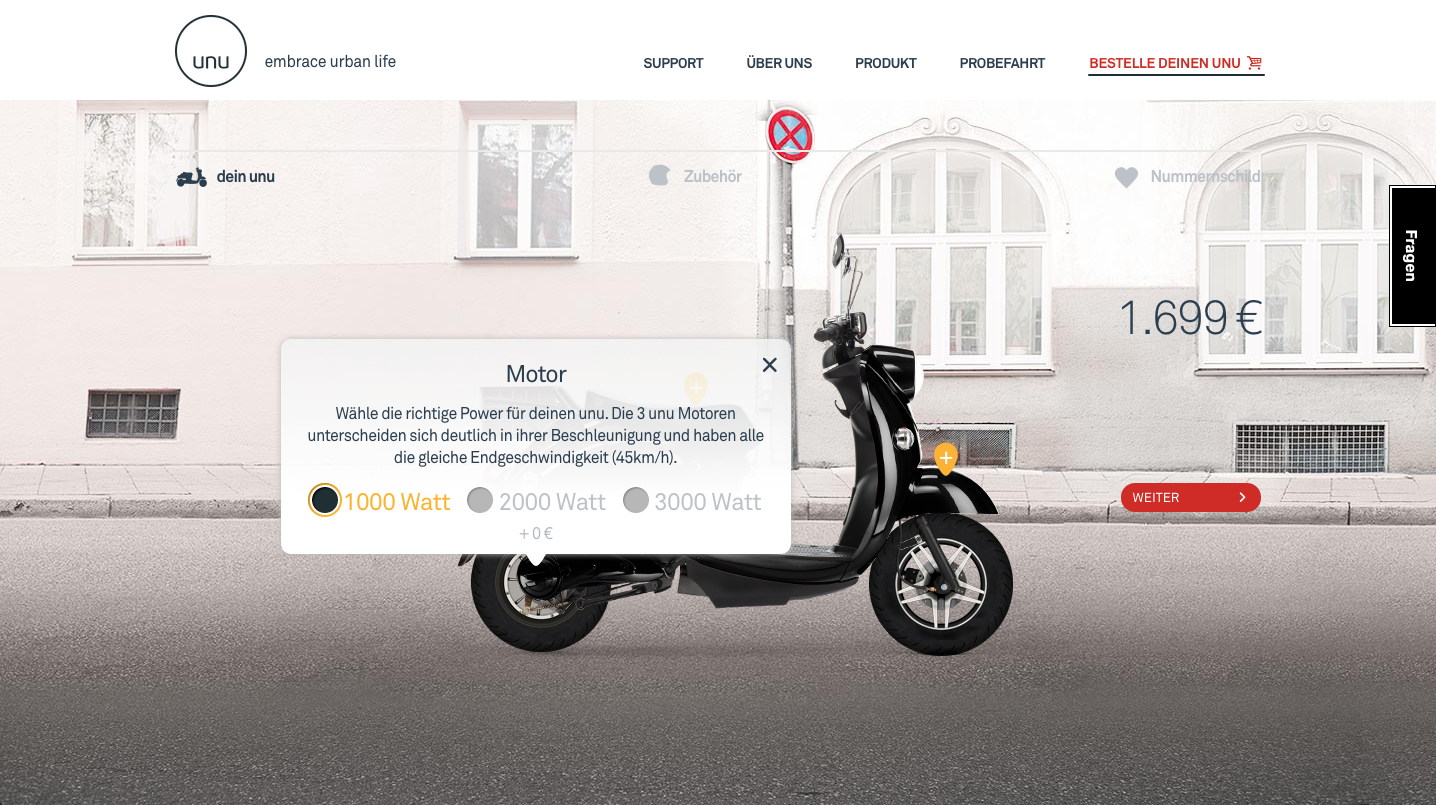
\includegraphics[width=\linewidth]{RelatedWork/img/unu-config}
  \caption{UNU GmbH\copyright{} electric scooter web configurator\cite{unu:2015:Online}}
\label{fig:unu-config}
\end{minipage}
\begin{minipage}{.45\textwidth}
\centering
  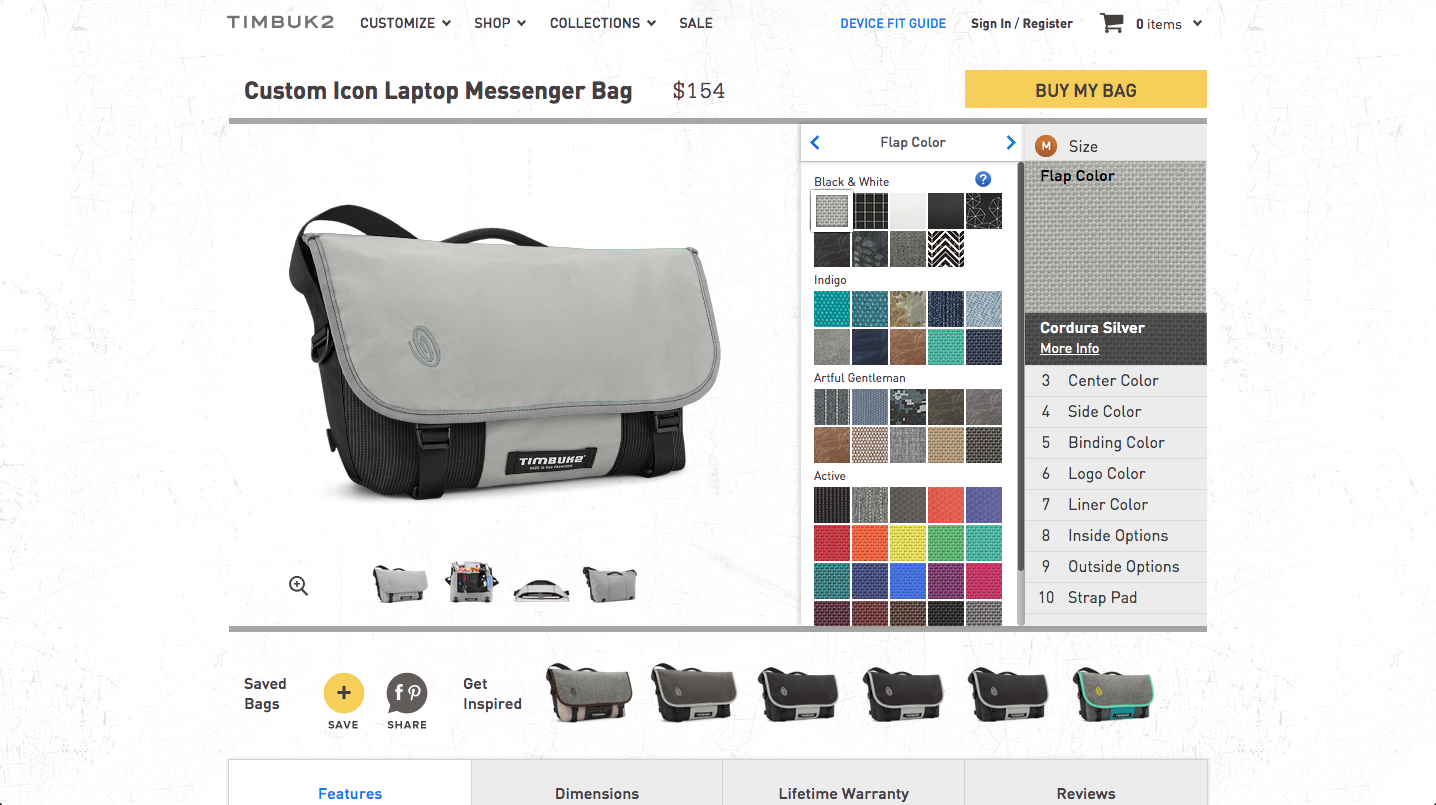
\includegraphics[width=\linewidth]{RelatedWork/img/timbuk2-config}
  \caption{Timbuk2\copyright{} bag web configurator\cite{timbuk2:2015:Online}}
\label{fig:timbuk2-config}
\end{minipage}
\end{figure}

\subsubsection{Gates 3D Configurator}
\subsubsection{Makervis}

\subsubsection{Twikit}

\subsection{Activity Sculptures}

\subsubsection{Sweet Atoms}

\subsubsection{Mental Fabrications}

\subsection{Activity Data Sources}

\subsubsection{Fitness Tracker APIs}
\end{document}
